\documentclass{amsart}
\usepackage{amsmath,amsthm}
\usepackage{graphicx}
\usepackage{wrapfig}
\usepackage{url}
\usepackage{caption}
\usepackage{subcaption}
\usepackage[justification=centering]{caption}

\usepackage{algorithm} % Must be loaded *after* hyperref
\usepackage[noend]{algpseudocode}

\title{The dynamics of factored state hidden Markov models}
\date{1 December 2020}

\begin{document}

\maketitle

\section{Introduction and Notation}\label{sec:intro}

\subsection{Classical hidden Markov models}
In what follows we denote random variables with upper case Latin letters like 
$X$, the probability distributions from which they are drawn with calligraphy 
letters like $\mathcal X$ and specific values with lower case Latin letters like $x$.  Suppose we have a sequence of observations, 
\[
X_{1:T} := X_1,...,X_T
\]
where at each time $t$, the observation $X_t$ can be decomposed into its 
categorical and continuous components, that is 
\begin{eqnarray}\label{eqn:decomposition}
X_t = W_t\oplus V_t
\end{eqnarray}
where $W_{t}$ is drawn from the categorical space
\[ 
\mathcal W = \{w_1,...,w_D\}
\]
and $V_t$ is drawn from a $K$ dimensional Gaussian distribution, $\mathbb R^K$.
A hidden Markov model (HMM) is a latent state model that captures the Markov dynamics of a latent process underlying the observed data.  In its most basic form, the HMM models a sequence of hidden states
\[
Z_{1:T} := Z_1,...,Z_T
\]
corresponding to $X_{1:T}$, where for any time $t$, the hidden state $Z_t$ is 
drawn from the discrete\footnote{Hidden states can of course be drawn from more complicated probability 
distributions -- see, for example, Chapter 13 of Bishop's canonical text on the 
topic \cite{B06}.  For sake of brevity, this note will only 
consider the discrete hidden state space.} probability distribution
\[
\mathcal{Z} = \{h_1,...,h_N\}.
\]
The sequence of hidden states satisfy the {\em Markov property}, that is 
\[
p(Z_t\mid Z_{t-1})=p(Z_t\mid Z_{t-1},Z_{t-2},...,Z_1),
\]
and therefore form a Markov chain.  A fully parameterized HMM, denoted by 
$\Theta$, is given by a set of three probability distributions: the initial state probability, the transition probability and the 
emission probability.

For a given $\Theta$, we assume 
these three distributions have a fixed, parametric form given by 
\begin{eqnarray*}
p(Z_1=z) &=& p_1(z;\theta_1)\\
p(Z_t = z\mid Z_{t-1}=z') & = & p_z(z\mid z';\theta_z)\\
p(X_t=x\mid Z_t=z) & = &p_x(x\mid z;\theta_x),
\end{eqnarray*} 
where 
\[
\Theta = \{\theta_1,\theta_z,\theta_x\}.
\]
For $X_t$ as in equation (\ref{eqn:decomposition}) we can refine this further, 
by
\begin{eqnarray*}
p_x(x\mid z;\theta_x)& = &p_{cat}(w\mid z; \theta_{cat})\cdot p_{cont}(v\mid z; \theta_{cont})
\end{eqnarray*}
for
\begin{eqnarray*}
p(W_t=w\mid Z_t=z) & = & p_{cat}(w\mid z; \theta_{cat}),\\
p(V_t=v\mid Z_t=z) & = & p_{cont}(v\mid z; \theta_{cont}),
\end{eqnarray*}
with $\theta_x = \{\theta_{cat},\theta_{cont}\}$.
The $\theta_i$ will often be left off of the expressions above when is clear 
from context. 

The {\em initial state probability} given by $p_1$ is encoded in an $N\times 1$ 
vector describing the probabilty of inhabiting each of the $N$ hidden states at 
time $t=1$.  The $i^{th}$ term of the initial state vector is given by  
$p_1(h_i; \theta_1)$. 

The {\em transition probability}, which describes the 
likelihood of transitioning from any one state to another, is captured in an 
$N\times N$ matrix, 
\[
A=\begin{bmatrix}
a_{ij}
\end{bmatrix}_{i,j=1}^N \text{ where }a_{ij} = p_z(h_j\mid h_i;\theta_z)
\]
One relevant observation that we can make about the transition matrix, is that 
every row of $A$ necessarily sums to 1, since 
\[
\sum_{j=1}^Np_z(h_j\mid h_i)=\sum_{j=1}^N\frac{p(h_j,h_i)}{p(h_i)}=1.
\]
marginal over $h_i$.

The {\em emission probability} is the parameter that directly 
couples the observation sequence and the hidden 
state sequence and captures the probability of an observation vector given each 
of the hidden states. The categorical part of the emission probability can be 
described by a $D\times N$ matrix, 
\[
B = \left[b_{i}(w_d)\right]_{d,i=1}^{D,N}\text{ where }b_{i}(w_d) =p_{cat}(w_d\mid h_i; \theta_{cat}).
\]
For the continuous part of the emission probability, each hidden state, $h_i$ 
corresponds to a $K$-dimensional Gaussian distribution with a 
$K$-dimensional mean vector, $\mu_i$, 
and $K\times K$ covariance matrix, $\Sigma_i$ for each hidden state $h_i$, and 
hence 
\[
p_{cont}(v\mid 
h_i;\theta_{cont})=\frac{\exp\left(-\frac{1}{2}\left(v-\mu_i\right)\Sigma_i^{-1}\left(v-\mu_i\right)^T\right)}{\sqrt{(2\pi)^K\mid \Sigma_i\mid}}.
\]
The graphical model for a classical HMM can 
be seen in Figure \ref{fig:HMM}.  One primary goal in much of what follows, will be to learn the components of 
$\theta$.

\begin{figure}
\centering
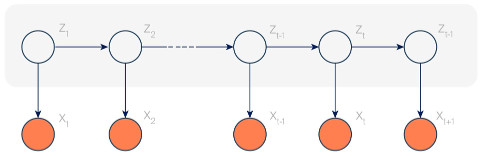
\includegraphics[scale=0.5]{figures/hmm.jpg}
\caption{The graphical model of a classical HMM}\label{fig:HMM}
\end{figure}

\subsection{Factored hidden Markov models}
In an fHMM with $M$ underlying Markov systems, the hidden state, $Z_t$, at time $t$, is an $M$-dimensional vector,
\[
Z_t = (Z_{t}^{(1)},...,Z_{t}^{(M)}),
\]
drawn from the probability distribution
\[
\mathcal Z = \mathcal{Z}^{(1)}\times ...\times \mathcal{Z}^{(M)}
\]
where 
\[
\mathcal Z^{(m)} = \{h_1^{(m)},...,h_{N_M}^{(m)}\}, 
\]
for all $1\leq m\leq M$.  To simplify the exposition, we will assume throughout this note that 
\[
N = N_1 = ...= N_M
\]
although a similar narrative will hold when this restiction is removed. 

The random variable $Z_t\in \mathcal Z$ can take on one of $N^M$ possible values, 
\begin{eqnarray}\label{eqn:vec}
s_i = (s_{i}^{(1)},...,s_{i}^{(M)})\text{ where }s_i^{(m)}\in \{h_1^{(m)},...,h_{N}^{(m)}\}
\end{eqnarray}
for $1\leq i\leq N^M$.  The set of hidden 
state variables in $\mathcal Z^{(m)}$ can be more concisely 
represented by a collection of $N$ 
many $N\times 1$ matrices, each 
of which is 0 in all but one component.  Therefore, we will represent the vector $s_i$ by a 
set of $M$ many $N\times1$ matrices corresponding to the appropriate 
$s_i^{(m)}$. A comprehensive treatment of fHMMs can be found in the foundational publication 
on the topic by Gharamani and Jordan \cite{GJ95}, but we will highlight some 
key components of that paper here.  

The full set of model parameters for an fHMM is 
still given by $\Theta$, with the additional factored state parameters 
\[
\theta_z = \{\theta_z^{(m)}:1\leq m \leq M\}.
\]
The initial state probability is given by 
a $1\times N^M$ vector since the initial state vector can take on one of $N^M$ values.  
The transition probability will now be described by a collection of $M$ many $N\times N$ matrices, 
\[
\{A^{(1)},...,A^{(M)}\},
\]
where 
\[
A^{(m)} = \begin{bmatrix}
a_{ij}^{(m)}
\end{bmatrix}_{1\leq i,j\leq N}\text{ where } a_{ij}^m = p_z(h_j^{(m)}\mid 
h_i^{(m)}; \theta_z^{(m)})
\]
for $1\leq m\leq M$.

The probability of transitioning from one hidden state vector to another can 
then be constructed as a tensor product of these matrices.  More concretely, 
the probabilty of transitioning from a particular hidden state vector at time 
$t-1$ to any another hidden state vector at time $t$ can be decomposed as the product
\begin{eqnarray}\label{eqn:trans2}
p(Z_t\mid Z_{t-1}) = \prod_{m=1}^M p(Z_{t}^{(m)} \mid Z_{t-1}^{(m)}).
\end{eqnarray}
In this way each of the Markov processes evolves independently, according to 
its own dynamics. A graphical model for the fHMM can be seen in Figure 
\ref{fig:fHMM}.

\begin{figure}
\centering
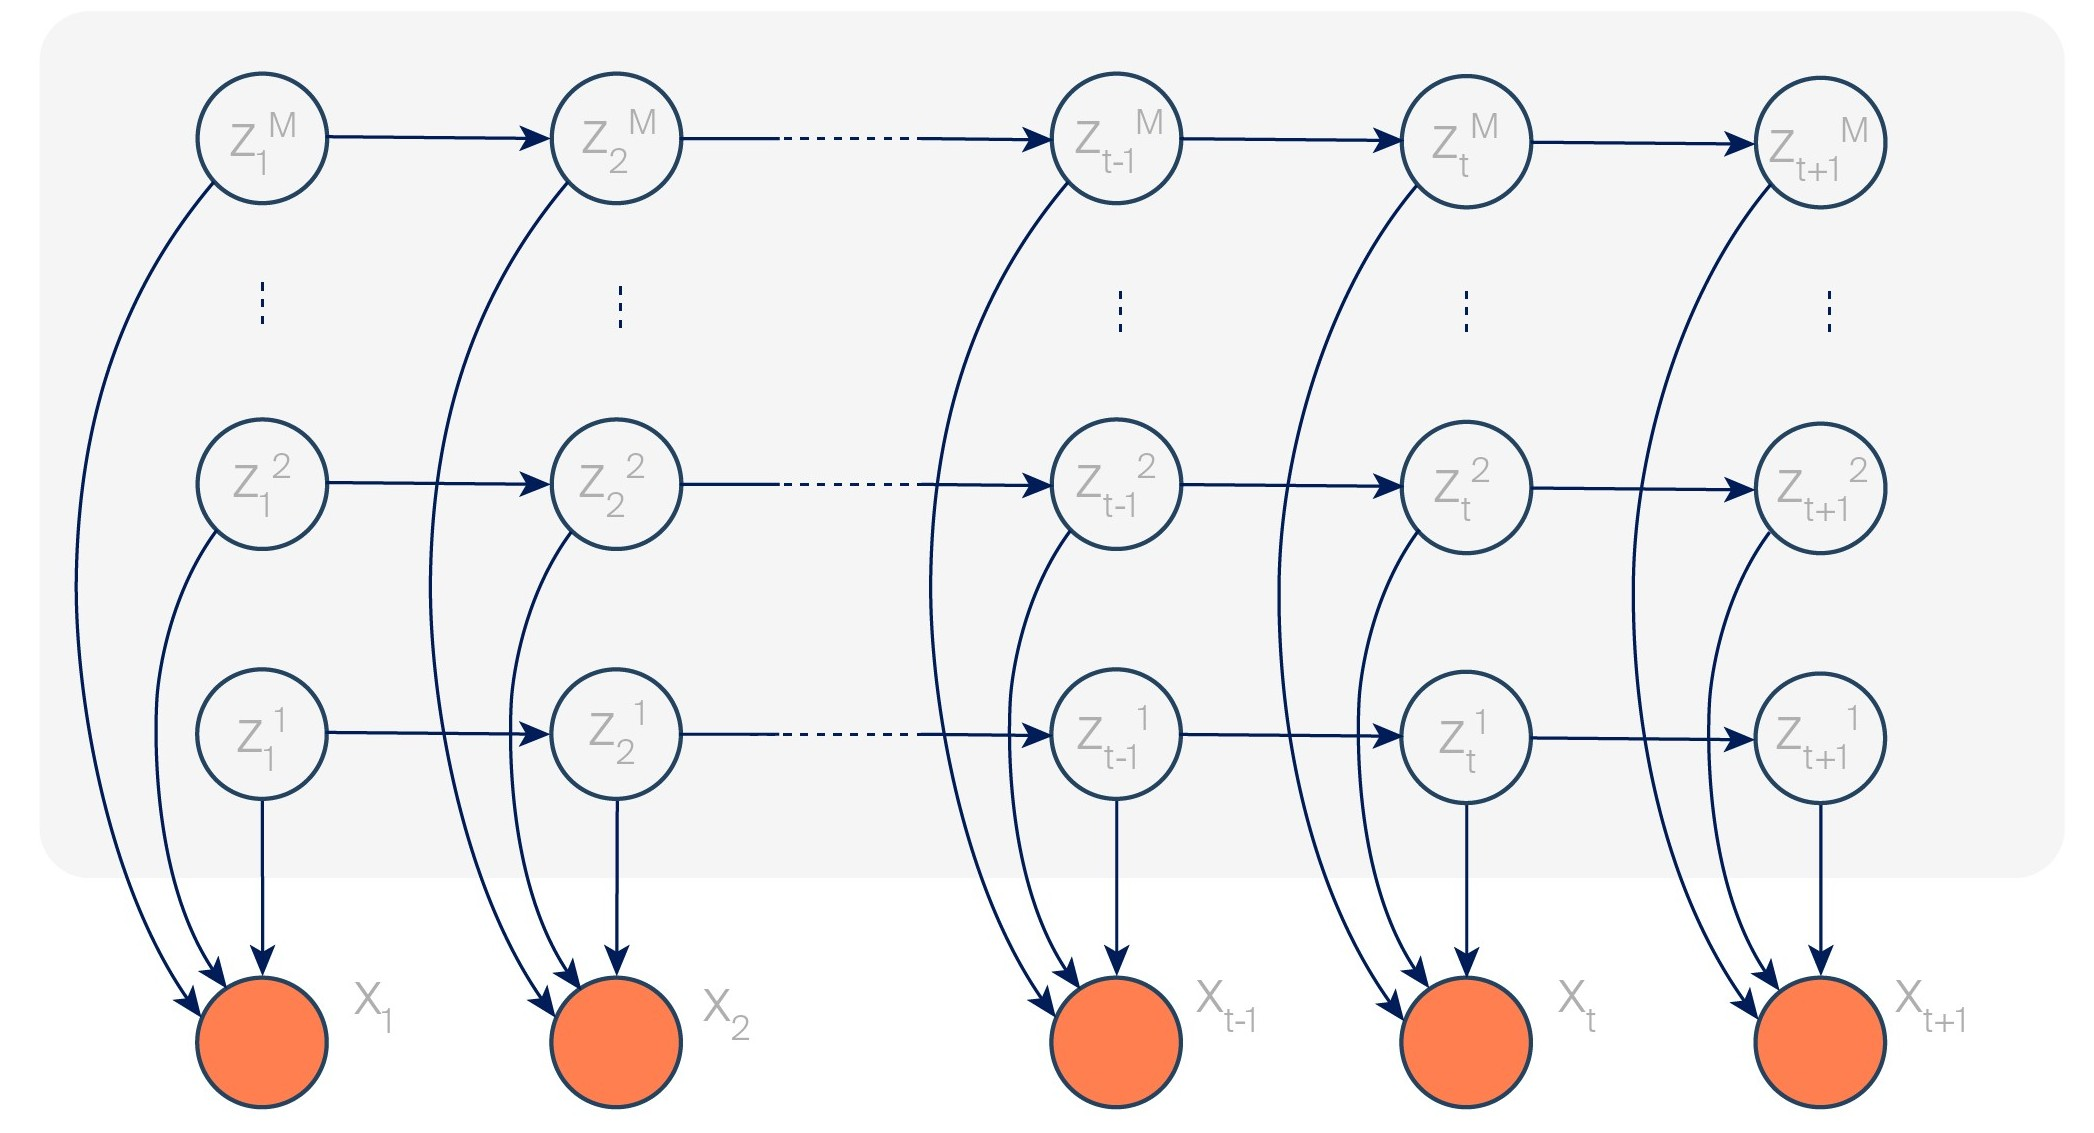
\includegraphics[scale=0.1]{figures/fhmm.jpg}
\caption{The graphical model of a factored HMM}\label{fig:fHMM}
\end{figure}

Although we want to maintain this marginal independence for the hidden states, 
$Z_{1:T}$, we would expect some dependence once we condition on the observation 
sequence, $X_{1:T}$.  To understand the intuition behind this, let's revisit our 
example of involving the five components of the wind turbine.  While we don't 
expect the status of the generator from time $t$ to $t+1$ to be connected to 
the status of the yaw motor from time $t$ to $t+1$, if we were to observe a 
power surge that causes the generator to experience a fault, that might 
increase the likelihood that the yaw motor experiences a fault\footnote{This is 
an example of what is known as ``Berkson's paradox".}.  If we consider 
the fHMM as a graphical model as in Figure (\ref{fig:fHMM}) we can couch this 
observation in the language of directed graphs and the so-called d-separation 
criterion. This conditional dependence means that, in particular, we would not expect the 
emission probability to decompose as a tensor product as in equation (\ref{eqn:trans2}). 

In the case of categorical observations we can 
describe the emission probability much like in the classical case, but encoding 
the information in a $D\times N^M$ matrix, $B$, where 
\[
B = \left[b_{i}(w_d)\right]_{d,i=1}^{D,N^M} \text{ where }b_{i}(w_d) = p_{cat}(w_d\mid 
s_i;\theta_{cat})
\]
The situation becomes more complicated for continuous observations.  In 
particular, the mean values for each Markov system and hidden state vector are 
given in a $K\times N$ matrix, $W^{(m)}$, where the $kn^{th}$ entry 
of $W^{(m)}$ is the contribution to the $k^{th}$ dimension by the $n^{th}$ 
hidden state vector for system $m$. For a hidden state vector, $s_i$, as in 
equation (\ref{eqn:vec}) we obtain a $K$-dimensional mean vector
\[
\mu_i = \sum_{m=1}^M W^{(m)}s_i^{(m)}
\]
which couples the hidden state vectors across the Markov systems.
Therefore, assuming a constant $K\times K$ covariance matrix, $\Sigma$, we have 
\[
p_{cont}(v\mid s_i;\theta_{cont}) = 
\frac{\exp\left(-\frac{1}{2}\left(v-\mu_i\right)\Sigma^{-1}\left(v-\mu_i\right)^T\right)}{\sqrt{(2\pi)^K\mid \Sigma\mid}}.
\]
This for a hidden state vector, $s_i$, and observation $x=w\oplus v$, we have
\begin{eqnarray}
p_x(x\mid s_i; \theta_x) = p_{cat}(w\mid 
s_i;\theta_{cat})\cdot p_{cont}(v\mid s_i;\theta_{cont}) .
\end{eqnarray}


\section{Learning and Inference for Factored HMMs}

\subsection{Flexible Gibbs Sampling for Factored HMMs}

In this section we will describe the components necessary to perform Gibbs 
sampling for fHMMs in a maximally flexible way following the notation set forth 
in Section \ref{sec:intro}.  Suppose we already know the model parameters, 
$\Theta$, then general strategy will be to determine the most 
likely sequence of hidden states for an observation sequence, $x_{1:T}$, by iterative 
sampling.  In particular, we will begin by randomly seeding a sequence of hidden 
states, $z_{1:T}$.  We will randomly traverse the full sequence, and for each time, 
$t$, and hidden state system, $m$, we will draw a sample  
\begin{equation}\label{eqn:sample}
{z_t^{(m)}}'\sim p(Z_t^{(m)}\mid \{z_t^{(n)}:n\neq m\},z_{t-1}^{(m)}, z_{t+1}^{(m)}, x_t),
\end{equation}
eventually replacing every $z_t^{(m)}$ with ${z_t^{(m)}}'$.  With sufficient 
iterations this process will eventually converge to a reasonable approximation 
for the most likely sequence of hidden states.  In order to do this, a first 
step will be to express equation (\ref{eqn:sample}) in terms of known 
quantities, $p_1,p_x$ and $p_z$.  By repeated applications of Bayes' rule and marginalizing over all possible hidden 
states for time $t$ and system $m$, we obtain 
\begin{eqnarray*}
&&p(Z_t^{(m)}\mid \{z_t^{(n)}:n\neq m\},z_{t-1}^{(m)}, z_{t+1}^{(m)}, x_t)\\
& = & \frac{
p(Z_t^{(m)},\{z_t^{(n)}:n\neq m\},z_{t-1}^{(m)}, z_{t+1}^{(m)}, x_t)
}{
\sum_{z\in \mathcal Z^{(m)}}p(z,\{z_t^{(n)}:n\neq m\},z_{t-1}^{(m)}, 
z_{t+1}^{(m)}, x_t)
}\\
& = & \frac{
p_x(x_t\mid Z_t^{(m)},\{z_t^{(n)}:n\neq m\})\cdot
p_z(z_{t+1}^{(m)}\mid Z_t^{(m)})\cdot
p_z(Z_t^{(m)}\mid z_{t-1}^{(m)})
}{
\sum_{z\in \mathcal Z^{(m)}}
p_x(x_t\mid z,\{z_t^{(n)}:n\neq m\})\cdot
p_z(z_{t+1}^{(m)}\mid z)\cdot
p_z(z\mid z_{t-1}^{(m)})
}.
\end{eqnarray*}
However, we can see the random variable $Z_t^{(m)}$ is independent of the 
denominator above, and therefore is not 
relevant to the sampling. Consequently, we can sample 
\begin{equation}\label{eqn:sample2}
z_t^{(m)}\sim p_x(x_t\mid Z_t^{(m)},\{z_t^{(n)}:n\neq m\})\cdot
p_z(z_{t+1}^{(m)}\mid Z_t^{(m)})\cdot
p_z(Z_t^{(m)}\mid z_{t-1}^{(m)}).
\end{equation}
For a fixed $x_{1:T}$ and $z_{1:T}$ we will denote this probabilty distribution 
in equation (\ref{eqn:sample2}) as a function 
\[
f_{t,m}:\mathcal Z^{(m)}\rightarrow \mathbb{R}
\]
where 
\[
f_{t,m}(z) := \begin{cases}
p_x(x_t\mid z,\{z_t^{(n)}:n\neq m\})\cdot
p_z(z_{t+1}^{(m)}\mid z)\cdot
p_1(z)& \text{ if }t=1\\
p_x(x_t\mid z,\{z_t^{(n)}:n\neq m\})\cdot
p_z(z_{t+1}^{(m)}\mid z)\cdot
p_z(z\mid z_{t-1}^{(m)})& \text{ if }1<t<T\\
p_x(x_t\mid z,\{z_t^{(n)}:n\neq m\})\cdot
p_z(z\mid z_{t-1}^{(m)})& \text{ if }t=T
\end{cases}
\]
The sampling This process is described in its totality in Algorithm \ref{alg:gibbs}.  


\begin{algorithm}
  \caption{Gibbs Sampling Algorithm\label{alg:gibbs}}
  \begin{algorithmic}[1]
    \Function{Gibbs}{model $p_0$, $p_x$, $p_z$; data $x_1,...,x_T$; hidden 
    state space $\mathcal Z$; iterations 
    $I$}
    \State $\tt{z}\leftarrow \{z_1,...,z_T\}$ initialized at random where 
    $\tt{z}_t=\{z_t^{(1)},...,z_t^{(M)})\}$
    \State ${\tt i}\leftarrow 0$
	\While{${\tt i}<I$}
      \For{all ${\tt t,m}$ in $\{0,\dots, 
      T\}\times \{0,\dots, M\}$ chosen uniformly at random} 
        \State ${\tt c} \leftarrow {\tt cumsum \{f_{t,m}(z):z\in \mathcal 
        Z^{(m)}\}}$ 
        \label{eqn:alg_prob}
        \State ${\tt u}\leftarrow$ an element of $[0,1]$ chosen uniformly at 
        random
        \State ${\tt j}\leftarrow$ minimum index of ${\tt c}$ for which 
        $\tt{u}\geq c_j$
        \State ${\tt z_t^{(m)}}\leftarrow {\tt j}^{th}$ element of $\mathcal Z^{(m)}$

      \EndFor
      \State ${\tt i}\leftarrow {\tt i+1}$
      \EndWhile
      \State\Return ${\tt z}$
    \EndFunction
  \end{algorithmic}
\end{algorithm}

\bibliographystyle{siam}
\bibliography{references}

\end{document}

